\documentclass[tikz,border=6pt]{standalone}
\usepackage{amsmath,amssymb}
\usepackage{xcolor}
\definecolor{accent}{HTML}{A13D2C}
\definecolor{accent2}{HTML}{2B5F6B}
\definecolor{muted}{HTML}{5A564F}
\definecolor{linecol}{HTML}{D8D2C4}
\definecolor{astroblue}{HTML}{1B4F72}
\usetikzlibrary{arrows.meta}
\IfFileExists{results/ch13/wd_MR.dat}{\def\datadir{results/ch13/}}{\def\datadir{../results/ch13/}}
\begin{document}
% White dwarfs: Newtonian equilibrium with the exact degenerate-electron pressure, mu_e = 2 (code/ch13/01_mass_radius.py).
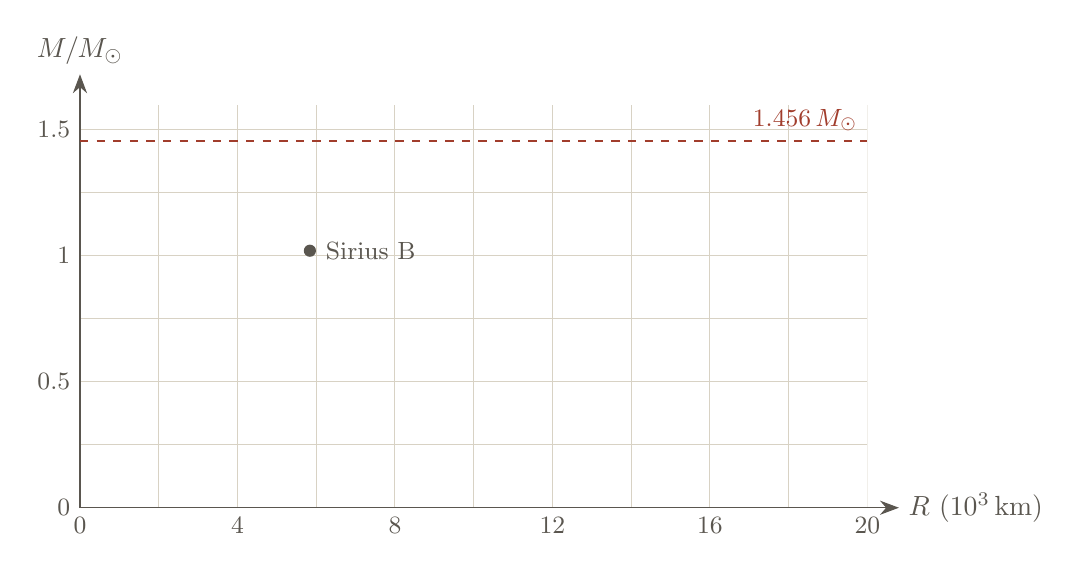
\begin{tikzpicture}[x=0.5cm,y=3.2cm, >={Stealth[length=2.4mm]}]
  \begin{scope}
    \clip (0,0) rectangle (20,1.6);
    \draw[linecol] (0,0) grid[xstep=2,ystep=0.25] (20,1.6);
    \draw[astroblue, line width=1.2pt] plot file {\datadir wd_MR.dat};
  \end{scope}
  \draw[->, muted] (0,0) -- (20.8,0) node[right] {$R\ (10^3\,\mathrm{km})$};
  \draw[->, muted] (0,0) -- (0,1.72) node[above] {$M/M_\odot$};
  \foreach \x in {0,4,8,12,16,20} \node[below, muted] at (\x,0) {\small \x};
  \foreach \y in {0,0.5,1,1.5} \node[left, muted] at (0,\y) {\small \y};
  \draw[accent, dashed, line width=0.9pt] (0,1.456) -- (20,1.456);
  \node[accent, above left] at (20,1.456) {\small $1.456\,M_\odot$};
  \fill[muted] (5.84,1.02) circle[radius=2.2pt];
  \node[muted, right] at (6.0,1.02) {\small Sirius B};
\end{tikzpicture}
\end{document}
